\section{Haftpflichtrecht}

Das Haftplfichtrecht unterscheided zwischen \textbf{vertraglicher} und
\textbf{ausservertrachlicher} Haftung / Culpa in contrahendo. Das Ziel des
Haftplichtrechtes ist es, \textbf{Schaden auszugleichen} sowie als
\textbf{Prävention} zu wirken.

\begin{figure}[H]
	\centering
	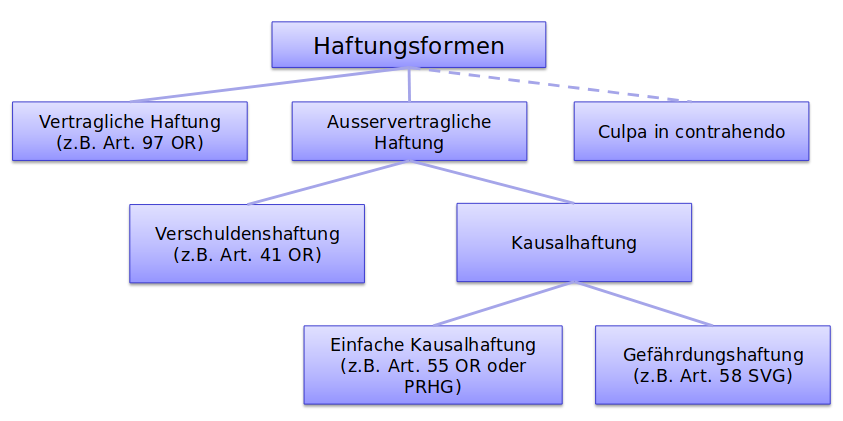
\includegraphics[width=.8\textwidth]{figures/haftpflichtrechtFormen.png}
	\caption{Formen der Haftpflicht}
\end{figure}


\subsection{Arten von ausservertraglichen Haftungen}
\label{sec:Haftpflicht-Arten}

\begin{description}
	\item[Verschuldungshaftung] Schädiger haftet grundsätzlich nur, wenn
	er den Eintritt des Schadens verschuldet hat (Persönliche
	Vorwerfbarkeit). (Art. 41 OR)
	\item[Kausalhaftung] Setzt kein Verschulden voraus, sondern ist
	gegeben, wenn durch das Gesetz festgelegte Tatbestandsvoraussetzungen
	erfüllt sind.
	\begin{itemize}
		\tightlist
		\item einfache Kausalhaftung
		\begin{itemize}
			\tightlist
			\item Geschäftsherrenhaftung (Art. 55 OR) - Chef haftet für Mitarbeiter
			\item Werkeigentümerhaftung (Art. 58 OR) - Haft für Werke (Baugerüste,
			Häuser, \ldots{})
			\item Haftung des Grundeigentümers (Art. 679 ZGB)
			\item Produktehaftpflicht (PrHG)
		\end{itemize}
		\item Gefährdungshaftung: Bestimmten Einrichtungen sind Gefahren inhärent,
		die den Betreibern dieser Einrichtungen eine besondere Verantwortung
		aufbürden (Gefahrensatz).
	\end{itemize}
\end{description}


\subsection{Voraussetzungen}

\begin{figure}[H]
	\centering
	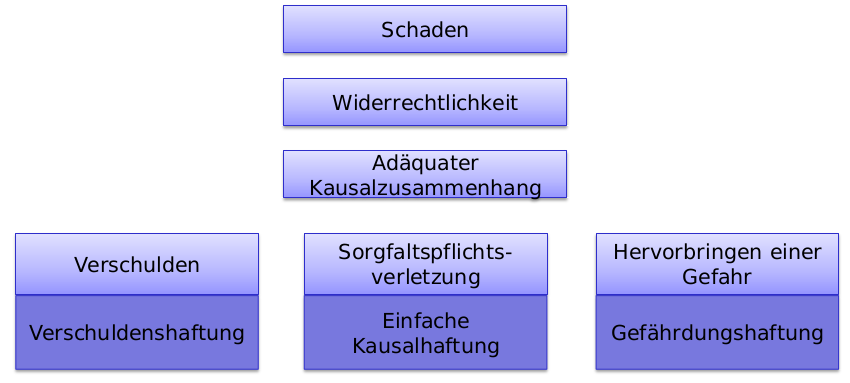
\includegraphics[width=.8\textwidth]{figures/haftpflichtVerschulden.png}
	\caption{Voraussetzungen bei Verschuldens- und Kausalhaftung}
\end{figure}

Folgende Punkte müssen \textbf{zwingend erfüllt sein}, damit eine Haftpflicht
vorliegt:

\begin{itemize}
\tightlist
\item Schaden
\item Wiederrechtlichkeit
\item Adäquater Kausalzusammenhang
\item Verschulden
\end{itemize}


\subsubsection{Definition Schaden (Vermögenseinbusse)}

Schaden ist eine unfreiwillige Verminderung des Vermögens in Form von:
\begin{itemize}
	\tightlist
	\item Abnahme der Aktiven
	\item Zunahme der Passiven
	\item Entgangener Gewinn
\end{itemize}

Der Schaden als Vermögenseinbusse bestimmt sich grundsätzlich nach
der \textbf{Differenz} zwischen dem gegenwärtigen Vermögensstand und dem Stand,
den das Vermögen ohne das schädigende Ereignis hätte.


\subsubsection{Schadensformen}

\begin{itemize}
	\tightlist
	\item Vermögensschaden
	\item Personenschaden (Beeinträchtigung der Gesundheit einer Person)
	\item Sachschaden (Wenn eine Sache Schaden nimmt, wie z.B. ein Laptop)
	\item Immaterieller Schaden (Reputation, Persönlichkeitsverletzung)
	\item Direkter Schaden (Der Schaden ist durch das schädige Ereignis direkt
	ausgelöst)
	\item Indirekter Schaden (Der Schaden entsteht später als das schädigende
	Ereignis)
\end{itemize}


\subsubsection{Definition Wiederrechtlichkeit}

\begin{itemize}
	\tightlist
	\item Es muss entweder ein absolutes Recht verletzt sein
	\begin{itemize}
		\tightlist
		\item Absolute Rechte sind Rechte, die gegenüber allen gelten
		\begin{itemize}
			\tightlist
			\item Besitz / Eigentum
			\item Leben
			\item Ehre
			\item Gesundheit
		\end{itemize}
	\end{itemize}
	\item Oder es muss eine Schutznom verletzt werden
	\begin{itemize}
		\tightlist
		\item Veruntreuung oder Datenbeschädigung
	\end{itemize}
\end{itemize}


\paragraph{Rechtfertigungsgründe}
\label{sec:Haftpflichtrecht-Rechtfertigung}
\begin{itemize}
	\tightlist
	\item Notwehr (Art. 52.1 OR) - Verhältnismässige Abwehr in einer
	Notsituation
	\item Notstand (Art. 52.2 OR) - Um sich selber zu schützen, greift man in
	das Rechtsgut eines anderen ein.
	\item Selbsthilfe (Art. 52.3 OR) - Die eigene Sache darf wieder veschaft
	werden (ohne Selbstjustiz)
	\item Einwilligung des Verletzten - z.B. eine Operation
	\item Amtspflicht - z.B. Taschenkontrolle durch einen Polizisten
\end{itemize}

\subsubsection{Definition: Adäquater Kausalzusammenhang}

Ein Kausalzusammenhang ist adäquat, wenn die betreffende Ursache
nach dem gewöhnlichen Lauf der Dinge und der allgemeinen
Lebenserfahrung an sich geeignet war, den eingetretenen Erfolg zu
bewirken, so dass der Eintritt dieses Erfolges als durch die fragliche
Tatsache allgemein begünstigt erscheint.\\
-> Schaden ist effektiv aus der Tat hervorgegangen.


\subsubsection{Verschuldungsformen}

\begin{description}
	\item[Vorsatz] Der Schuldner strebt einen Erfolg bewusst an.
	\item[Eventualvorsatz] Der Schädiger nimmt ein Schaden in Kauf.
	\item[Fahrlässigkeit] Nicht absichtlich angestrebte
	\emph{mangelhafte Sorgfalt} führt zur Verletzung.\\
	Kriterium: Durchschnittliches Verhalten eines
	vernünftigen und ordentlichen Menschen.
	\begin{description}
		\tightlist
		\item[Grobe Fahrlässigkeit] Die gebotene Sorgfaltspflicht ist in
		besonders schwerer Weise verletzt.
		\item[Leichte Fahrlässigkeit] Das Verhalten des Schädigers kann
		als ``einigermassen verständlich'' bezeichnet werden. z.B. wenn man
		aus Versehen jemand mit einer Dampfwalze überfährt
	\end{description}
\end{description}

\subsection{Beweislast}

\begin{figure}[H]
	\centering
	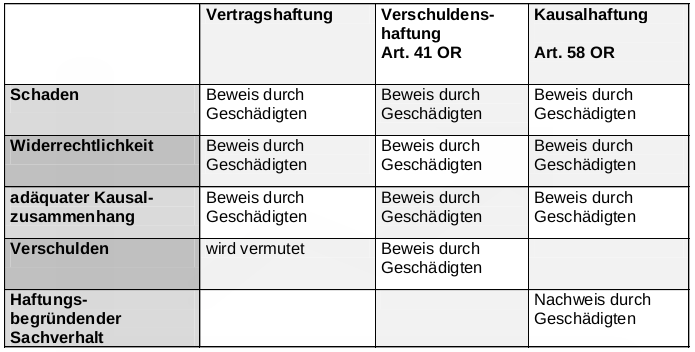
\includegraphics[width=.8\textwidth]{figures/Voraussetzungen_Haftpflichtrecht.png}
	\caption{Beweislast bei den verschiedenen Haftungstypen}
\end{figure}



\subsection{Werkeigentümerhaftpflicht}

Ihrem Unternehmen gehört eine Lokalität im Herzen der Altstadt von
Liestal. Herr X, interessiert sich für Ihre Produkte, die er im
Schaufenster sieht und möchte Ihren Laden betreten. Er rutscht auf dem
Eis vor der Ausgangstüre aus und verletzt sich am Knöchel. Liegt hier
ein Fall der Werkeigentümerhaftpflicht vor? (Art. 58 OR)

\begin{itemize}
	\tightlist
	\item Schaden: Der Knöchel ging defekt, der Arzt kostet
	\item Verschulden: Mangelhafte Unterhaltung des Werkes
	\item Wiederrechtlichkeit: Unbetrittenes Recht für Gesundheit wurde
	verletzt
	\item Werk: Alles, was künstlich hergestellt und mit dem Boden verbunden ist
	\item Vorliegen eines Werkmangels: Werk bietet bei bestimmungsgemässen
	Gebrauch keine genügende Sicherheit
	\item Kausalzusammenhang
	\item Mangelnder Unterhalt
	\item BGer: ``Wer den Besuchern eines Verkaufslokals eine Ausgangstüre zur
	Verfügung stellt, hat für deren möglichst gefahrlose Benützbarkeit zu
	sorgen. Dazu gehört auch, dass er unmittelbar jenseits der Türe
	laufende Gefahren, wie Glatteis auf dem Trottoir, im Rahmen des
	Möglichen und Zumutbaren beseitigt oder zumindest mit einem Warnschild
	(Achtung gschliferig) darauf aufmerksam macht.''
\end{itemize}

\subsection{Produktehaftpflichtgesetz}

\begin{figure}[H]
	\centering
	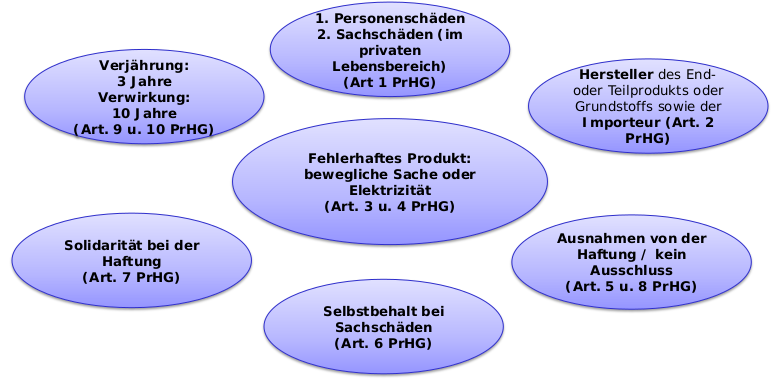
\includegraphics[width=.8\textwidth]{figures/produkthaftpflicht.png}
	\caption{Privathaftpflichtgesetz}
\end{figure}

\begin{itemize}
	\tightlist
	\item Der Schaden an Personen ist gedeckt
	\item Private Sachschäden sind auch gedeckt. Werden jedoch Dinge von einem
	Unternehmen beschädigt, ist dies nicht gedeckt.
	\item Produkthaftpflicht darf nicht durch AGBs oder andere Verträge
	ausgeschlossen werden
	\item Solidarität bei der Haftung heisst: Auch wenn man als Importeur z.B.
	nichts für das Versagen des Produkts hat, haftet man und muss zahlen.
	\item Die Produktehaftpflicht gilt nur 10 Jahre nach Einführung des Produkts
	und 3 Jahre nach Eintritt eines Schadens
\end{itemize}

\subsection{Gefährdungshaftung}
\label{sec:Haftpflicht-Gefaerdungshaftung}
Die Gefährdungshaftung ist eine qualifizierte Kausalhaftung, indem sie
davon ausgeht, dass bestimmten Einrichtungen Gefahren inhärent sind, die
den Betreibern dieser Einrichtungen eine besondere Verantwortung
aufbürden.\\
BSP: Haftpflicht des Motorfahrzeughalters (SVG)

\paragraph{Art. 58.1 SVG}
Wird durch den Betrieb eines Motorfahrzeuges ein Mensch getötet oder
verletzt oder Sachschaden verursacht, so haftet der Halter für den
Schaden.


\subsection{Culpa in contrahendo}

Ist im Gesetz nirgends geregelt.

„Verschulden bei Vertragsverhandlung`` Voraussetzungen:

\begin{itemize}
	\tightlist
	\item es werden Verhandlungen über einen zukünftigen Vertrag geführt,
	\item vorvertragliche Pflichten werden verletzt,
	\item eine der Vertragsparteien erleidet einen Schaden, welcher
	\item adäquat-kausal aus der Pflichtverletzung hervorgeht
	\item und dem Verschulden der schädigenden Person zuzuschreiben ist.
\end{itemize}
